\subsubsection{Explicación}
El recorrido parcial inicial lo determinan los 3 puntos que estén más al Este, Oeste y Norte respectivamente. La única restricción es que los 3 no sean los mismos, algo que nunca pasa, pues 2 de ellos pueden ser iguales (un punto puede ser a la vez el punto más al Norte y al Este), pero 3 a la vez no.

EL nodo siguiente a insertar en el recorrido parcial será un nodo arbitrario, de lo que nos encargaremos para hacer funcionar el greedy es de insertarlo entre los dos vértices que más convengan, minimizar la distancia del circuito resultante.

Pasaremos por todos los vértices que nos quedan cada vez, y sobre cada uno calculamos la posición que más nos convenga dentro del circuito, y luego escogemos el vértice que nos da mejor resultado.

\subsubsection{Eficiencia}
Tenemos que recorrer $n$ vértices, y sobre cada uno de ellos aplicaremos una función $\phi(x)$ para cada vértice.

\[ \sum_{i=1}^{n} \phi(x_i)\]

Dicha función $\phi(x)$ llama a "buscar punto" que es lineal, cada vez que buscas un punto llama $n$ veces a "buscar posicion", que a su vez llama $n$ veces a calcular longitud.

Por tanto $\phi(x)$ es cúbica, y la eficiencia que nos queda para el algoritmo de inserción es
\[ O(n) = n^4 \]

\newpage
\subsubsection{Ejemplos}
Puntos:

	\begin{figure}[htbH]
		\centering
		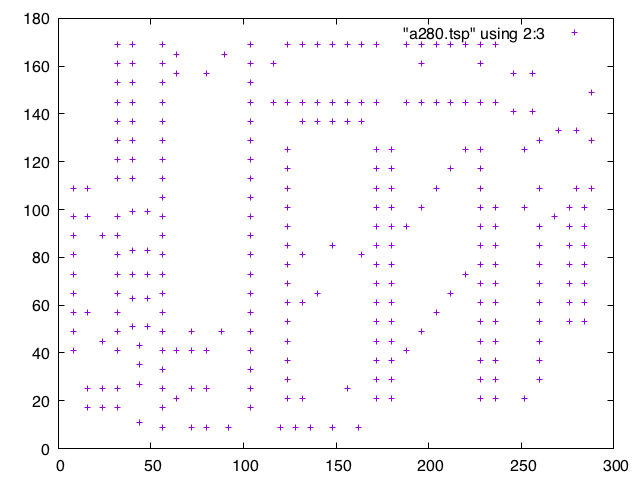
\includegraphics[width=0.65\textwidth]{../Viajante/Imagenes/a280.png}
		\caption{Quinto vértice}
	\end{figure}
	
Recorrido óptimo:

	\begin{figure}[htbH]
		\centering
		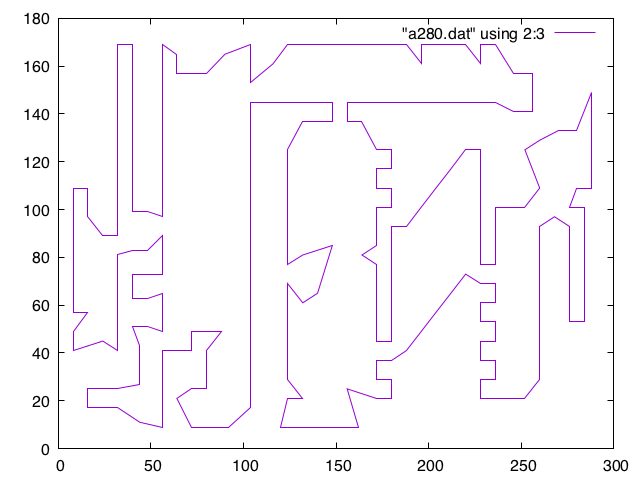
\includegraphics[width=0.65\textwidth]{../Viajante/Imagenes/a280_opt.png}
		\caption{Quinto vértice}
	\end{figure}
\newpage